%\documentclass[tikz,convert={outfile=jobname.svg}]{standalone}
\documentclass[border=1pt, multi=page]{standalone}

\pdfoutput=1

\usepackage{amssymb}
\usepackage{amsmath}
\usepackage{mathdots}
\usepackage{verbatim}
\usepackage[utf8]{inputenc}
%
\usepackage[all]{xy}
\usepackage{graphicx}
\usepackage{lmodern}

\usepackage{mathrsfs}

\usepackage{tikz}
\usepackage[europeanresistors, americaninductors, europeanvoltages, europeancurrents]{circuitikz}
%\usepackage[european]{circuitikz}

%\textwidth=19 truecm
%\textheight=26 truecm
%\hoffset=-3.5 truecm
%\voffset=-2.5 truecm

\newcommand{\ud}{\mathrm{d}}

\begin{document}

\begin{page}
	\begin{circuitikz}
		\ctikzset{bipoles/thickness=1.0}
		\tikzstyle{every node}=[font=\normalsize]

		\draw [line width=1pt](0,0) to[L,l_={$L$}] (0,2);
		\draw [line width=1pt](3,0) to[C,l^={$C$}] (3,2);
		\draw [line width=1pt](0,0) to[short] (3,0);
		\draw [line width=1pt](0,2) to[short] (3,2);
	\end{circuitikz}
\end{page}

\begin{page}
	\begin{circuitikz}
		\ctikzset{bipoles/thickness=1}
		\tikzstyle{every node}=[font=\normalsize]
		
		\draw [line width=1pt] (0,0) to[barrier, name=JJ] (3,0);
		\node[below=5mm, anchor=center, black] at (JJ) {$E_J$};
		
	\end{circuitikz}
\end{page}

\begin{page}
	\begin{circuitikz}
		\ctikzset{bipoles/thickness=1.0}
		\tikzstyle{every node}=[font=\normalsize]
		
		%\node[below=3mm, anchor=center, black] at (JJ) {$E_J$};
		
		\draw [line width=1pt](0,0) to[barrier, name=JJ, l_={\hspace{-0.25cm}$E_J$}] (0,2);
		\draw [line width=1pt](3,0) to[C,l^={$C_J$} ] (3,2);
		\draw [line width=1pt](0,0) to[short] (3,0);
		\draw [line width=1pt](0,2) to[short] (3,2);
		
        \draw [line width=1pt](1.5,0) to[short, *-] (1.5,-1);
		\draw [line width=1pt](1.5,2) to[short, *-] (1.5,3);

        \draw [line width=1pt](6,0) to[short, -] (6,-1);
		\draw [line width=1pt](6,2) to[short, -] (6,3);
		\draw [line width=1pt](6,0) -- (6,0.75);
		\draw [line width=1pt](6,1.25) -- (6,2);
		\draw [line width=1pt](5.75,0.75) -- (6.25, 1.25);
		\draw [line width=1pt](5.75, 1.25) -- (6.25, 0.75);
		\draw [line width=1pt](5.75,0.75) rectangle (6.25, 1.25);

		
	\end{circuitikz}
\end{page}

\begin{page}
	\begin{circuitikz}
		\ctikzset{bipoles/thickness=1.0}
		\tikzstyle{every node}=[font=\normalsize]
		
		%\node[below=3mm, anchor=center, black] at (JJ) {$E_J$};
		
		\draw [line width=1pt](0,0) to[barrier, name=JJ, l_={\hspace{-0.25cm}$E_J$}] (0,2);
		\draw [line width=1pt](3,0) to[C,l^={$C_J$} ] (3,2);
		\draw [line width=1pt](0,0) to[short] (3,0);
		\draw [line width=1pt](0,2) to[short] (3,2);
		
		\draw [line width=1pt](1.5,0) to[short, *-*] (1.5,-1);
		\draw [line width=1pt](1.5,2) to[short, *-] (1.5,3);
		
		\draw [line width=1pt](1.5,-1) to[short] (6,-1);
		\draw [line width=1pt](1.5,3) to[short] (6,3);
		\draw [line width=1pt](6,-1) to[short] (6,3);
		\draw [line width=1pt](1.5,-1) to (1.5,-1.49);
		\draw [line width=0.7pt](1.5,-1.49) to (1.5,-1.5) node[tlground]{};
	\end{circuitikz}
\end{page}

\begin{page}
	\begin{circuitikz}
		\ctikzset{bipoles/thickness=1.0}
		\tikzstyle{every node}=[font=\normalsize]
		
		%\node[below=3mm, anchor=center, black] at (JJ) {$E_J$};
		
		\draw [line width=1pt](0,0) to[barrier, name=JJ, l_={\hspace{-0.25cm}$E_J$}] (0,2);
		\draw [line width=1pt](3,0) to[C,l^={$C_J$} ] (3,2);
		\draw [line width=1pt](0,0) to[short] (3,0);
		\draw [line width=1pt](0,2) to[short] (3,2);
		
		\draw [line width=1pt](1.5,0) to[short, *-*] (1.5,-1);
		\draw [line width=1pt](1.5,2) to[short, *-] (1.5,3);
		
		\draw [line width=1pt](1.5,-1) to[short] (6,-1);
		\draw [line width=1pt](1.5,3) to[short] (6,3);
		\draw [line width=1pt](6,-1) to[ammeter, l^={$I_0 \sin\phi$}] (6,3);
		\draw [line width=1pt](1.5,-1) to (1.5,-1.49);
		\draw [line width=0.7pt](1.5,-1.49) to (1.5,-1.5) node[tlground]{};
	\end{circuitikz}
\end{page}


\begin{page}
	\begin{circuitikz}
		\ctikzset{bipoles/thickness=1.0}
		\tikzstyle{every node}=[font=\normalsize]
		
		%\node[below=3mm, anchor=center, black] at (JJ) {$E_J$};
		
		\draw [line width=1pt](0,0) to[barrier, name=JJ, l_={\hspace{-0.25cm}$E_J$}] (0,2);
		\draw [line width=1pt](3,0) to[C,l^={$C_J$} ] (3,2);
		\draw [line width=1pt](0,0) to[short] (3,0);
		\draw [line width=1pt](0,2) to[short] (3,2);
		
		\draw [line width=1pt](1.5,0) to[short, *-*] (1.5,-1);
		\draw [line width=1pt](1.5,2) to[short, *-] (1.5,3);
		
		\draw [line width=1pt](1.5,-1) to[short] (6,-1);
		\draw [line width=1pt](1.5,3) to[short] (6,3);
		\draw [line width=1pt](6,-1) to[isource, l^={$I$}] (6,3);
		\draw [line width=1pt](1.5,-1) to (1.5,-1.49);
		\draw [line width=0.7pt](1.5,-1.49) to (1.5,-1.5) node[tlground]{};
	\end{circuitikz}
\end{page}

\begin{page}
	\begin{circuitikz}
		\ctikzset{bipoles/thickness=1.0}
		\tikzstyle{every node}=[font=\normalsize]
		
		%\node[below=3mm, anchor=center, black] at (JJ) {$E_J$};
		
		\draw [line width=1pt](0,0) to[barrier, name=JJ, l_={\hspace{-0.25cm}$E_J$}] (0,2);
		\draw [line width=1pt](3,0) to[C,l^={$C_J$} ] (3,2);
		\draw [line width=1pt](0,0) to[short] (3,0);
		\draw [line width=1pt](0,2) to[short] (3,2);
		
		\draw [line width=1pt](1.5,0) to[short, *-*] (1.5,-1);
		\draw [line width=1pt](1.5,2) to[short, *-] (1.5,3);
		
		\draw [line width=1pt](1.5,-1) to[short] (6,-1);
		\draw [line width=1pt](1.5,3) to[C,l_={$C_g$}] (6,3);
		\draw [line width=1pt](6,-1) to[vsource, l^={$V_g$}] (6,3);
		\draw [line width=1pt](1.5,-1) to (1.5,-1.49);
		\draw [line width=0.7pt](1.5,-1.49) to (1.5,-1.5) node[tlground]{};
	\end{circuitikz}
\end{page}

\begin{page}
	\begin{circuitikz}
		\ctikzset{bipoles/thickness=1.0}
		\tikzstyle{every node}=[font=\normalsize]
		
		%\node[below=3mm, anchor=center, black] at (JJ) {$E_J$};
		
		\draw [line width=1pt](1.5,0) to[C,l^={$C_J$} ] (1.5,2);
		
		\draw [line width=1pt](1.5,0) to[short, -*] (1.5,-1);
		\draw [line width=1pt](1.5,2) to[short, -] (1.5,3);
		
		\draw [line width=1pt](1.5,-1) to[short] (6,-1);
		\draw [line width=1pt](1.5,3) to[C,l_={$C_g$}] (6,3);
		\draw [line width=1pt](6,-1) to[vsource, l^={$V_g$}] (6,3);
		\draw [line width=1pt](1.5,-1) to (1.5,-1.49);
		\draw [line width=0.7pt](1.5,-1.49) to (1.5,-1.5) node[tlground]{};
	\end{circuitikz}
\end{page}



\begin{page}
	\begin{circuitikz}
		\ctikzset{bipoles/thickness=1.0}
		\tikzstyle{every node}=[font=\normalsize]
		
		%\node[below=3mm, anchor=center, black] at (JJ) {$E_J$};
		
		\draw [line width=1pt](0,0) to[barrier, name=JJ1] (0,2);
		\node[below=12, right=12, anchor=center, black] at (JJ1) {$E_{J,1}$};

		\draw [line width=1pt](1.5,0) to[barrier, name=JJ2] (1.5,2);
		\node[above=12, left=12, anchor=center, black] at (JJ2) {$E_{J,2}$};
		\node[] at (0.75, 1) {$\tilde\Phi$};
		
		\draw [line width=1pt](3,0) to[C,l^={$C_J$} ] (3,2);
		\draw [line width=1pt](0,0) to[short] (3,0);
		\draw [line width=1pt](0,2) to[short] (3,2);
		
		\draw [line width=1pt](1.5,0) to[short, *-*] (1.5,-1);
		\draw [line width=1pt](1.5,2) to[short, *-] (1.5,3);
		
		\draw [line width=1pt](1.5,-1) to[short] (6,-1);
		\draw [line width=1pt](1.5,3) to[C,l_={$C_g$}] (6,3);
		\draw [line width=1pt](6,-1) to[vsource, l^={$V_g$}] (6,3);
		\draw [line width=1pt](1.5,-1) to (1.5,-1.49);
		\draw [line width=0.7pt](1.5,-1.49) to (1.5,-1.5) node[tlground]{};
	\end{circuitikz}
\end{page}

\begin{page}
	\begin{circuitikz}
		\ctikzset{bipoles/thickness=1.0}
		\tikzstyle{every node}=[font=\normalsize]
		
		%\node[below=3mm, anchor=center, black] at (JJ) {$E_J$};
		
		\draw [line width=1pt](0,0) to[barrier, name=JJ, l_={\hspace{-0.25cm}$E_J$}] (0,2);
		\draw [line width=1pt](3,0) to[C,l^={$C_J$} ] (3,2);
		\draw [line width=1pt](0,0) to[short] (3,0);
		\draw [line width=1pt](0,2) to[short] (3,2);
		
		\draw [line width=1pt](1.5,0) to[short, *-*] (1.5,-1);
		\draw [line width=1pt](1.5,2) to[short, *-] (1.5,3);
		\draw [line width=1pt](1.5,-1) to[short] (6,-1);
		\draw [line width=1pt](1.5,3) -- (3.75,3);
		\draw [line width=1pt](3.75,3) to[C,l_={$C_g$}] (6,3);
		\draw [line width=1pt](6,-1) to[vsource, l^={$V_g$}] (6,3);
		\draw [line width=1pt](1.5,-1) to (1.5,-1.49);
		\draw [line width=0.7pt](1.5,-1.49) to (1.5,-1.5) node[tlground]{};
		
		\draw [line width=1pt](3.75,-1) to[C, l_={$C_B$}, *-] (3.75,0);
		\draw [line width=1pt](3.75,0) to[short, -*] (3.75,3);
	\end{circuitikz}
\end{page}

\begin{page}
	
\begin{tikzpicture}[thick,scale=2, every node/.style={scale=2}]
        \fill [fill=gray!50!white](0,0) rectangle (3,1);
        \fill [fill=purple!50!white](3,0) rectangle (3.5,1);
        \fill [fill=gray!50!white](3.5,0) rectangle (6.5,1);
        
        \fill [fill=gray!90!white](0,1) -- (3,1) -- (3.75,1.35) -- (0.75,1.35) -- cycle;
        \fill [fill=purple!30!gray](3,1) -- (3.5,1) -- (4.25,1.35) -- (3.75,1.35) -- cycle;
        \fill [fill=gray!90!white](3.5,1) -- (6.5,1) -- (7.25,1.35) -- (4.25,1.35) -- cycle;
        
        \fill [fill=gray!20!white](6.5,0) -- (7.25,0.35) -- (7.25,1.35) -- (6.5,1) -- cycle;
        
		\node[] at (1.5, 0.5) {\tiny superconductor};
		\node[] at (5.0, 0.5) {\tiny superconductor};
		\node[] at (3.25, -0.15) {\tiny insulator};
		
		\draw[<->, name=arrow] (3,0.5) -- (3.5,0.5);
		\node[] at (3.25,0.75) {{\fontsize{3.5}{5.5}\selectfont $1\,nm$}};
	\end{tikzpicture}
\end{page}

\begin{page}
	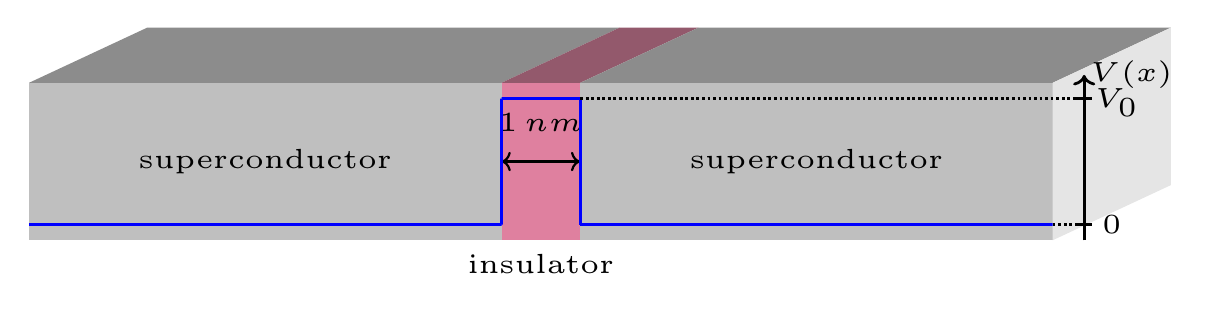
\begin{tikzpicture}[thick,scale=2, every node/.style={scale=2}]
        \fill [fill=gray!50!white](0,0) rectangle (3,1);
        \fill [fill=purple!50!white](3,0) rectangle (3.5,1);
        \fill [fill=gray!50!white](3.5,0) rectangle (6.5,1);
        
        \fill [fill=gray!90!white](0,1) -- (3,1) -- (3.75,1.35) -- (0.75,1.35) -- cycle;
        \fill [fill=purple!30!gray](3,1) -- (3.5,1) -- (4.25,1.35) -- (3.75,1.35) -- cycle;
        \fill [fill=gray!90!white](3.5,1) -- (6.5,1) -- (7.25,1.35) -- (4.25,1.35) -- cycle;
        
        \fill [fill=gray!20!white](6.5,0) -- (7.25,0.35) -- (7.25,1.35) -- (6.5,1) -- cycle;
        
		\node[] at (1.5, 0.5) {\tiny superconductor};
		\node[] at (5.0, 0.5) {\tiny superconductor};
		\node[] at (3.25, -0.15) {\tiny insulator};
		
		\draw[<->, name=arrow] (3,0.5) -- (3.5,0.5);
		\node[] at (3.25,0.75) {{\fontsize{3.5}{5.5}\selectfont $1\,nm$}};
		
		\draw [line width=1pt, color=blue](0,0.1) to[short, -] (3,0.1);
		\draw [line width=1pt, color=blue](3.0,0.1) to[short, -] (3.0,0.9);
		\draw [line width=1pt, color=blue](3.0,0.9) to[short, -] (3.5,0.9);
		\draw [line width=1pt, color=blue](3.5,0.1) to[short, -] (3.5,0.9);
        \draw [line width=1pt, color=blue](3.5,0.1) to[short, -] (6.5,0.1);
        
   		\draw [->, line width=1pt, name=yaxis](6.7,0) -- (6.7,1.05);
		\node[] at (7,1.05) {{\fontsize{3.5}{5.5}\selectfont $V(x)$}};
   		\draw [-, line width=1pt](6.65,0.1) -- (6.75,0.1);
		\node[] at (6.875,0.1) {{\fontsize{3.5}{5.5}\selectfont $0$}};
   		\draw [-, line width=1pt](6.65,0.9) -- (6.75,0.9);
		\node[] at (6.91,0.875) {{\fontsize{3.5}{5.5}\selectfont $V_0$}};

   		\draw [-, line width=1pt, densely dotted](6.5,0.1) -- (6.65,0.1);
   		\draw [-, line width=1pt, densely dotted](3.5,0.9) -- (6.65,0.9);

		
	\end{tikzpicture}
\end{page}


\begin{page}
	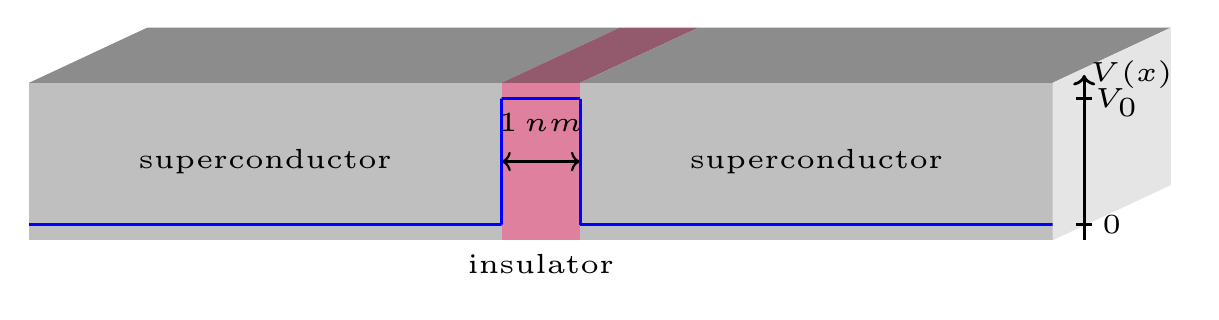
\begin{tikzpicture}[thick,scale=2, every node/.style={scale=2}]
        \fill [fill=gray!50!white](0,0) rectangle (3,1);
        \fill [fill=purple!50!white](3,0) rectangle (3.5,1);
        \fill [fill=gray!50!white](3.5,0) rectangle (6.5,1);
        
        \fill [fill=gray!90!white](0,1) -- (3,1) -- (3.75,1.35) -- (0.75,1.35) -- cycle;
        \fill [fill=purple!30!gray](3,1) -- (3.5,1) -- (4.25,1.35) -- (3.75,1.35) -- cycle;
        \fill [fill=gray!90!white](3.5,1) -- (6.5,1) -- (7.25,1.35) -- (4.25,1.35) -- cycle;
        
        \fill [fill=gray!20!white](6.5,0) -- (7.25,0.35) -- (7.25,1.35) -- (6.5,1) -- cycle;
        
		\node[] at (1.5, 0.5) {\tiny superconductor};
		\node[] at (5.0, 0.5) {\tiny superconductor};
		\node[] at (3.25, -0.15) {\tiny insulator};
		
		\draw[<->, name=arrow] (3,0.5) -- (3.5,0.5);
		\node[] at (3.25,0.75) {{\fontsize{3.5}{5.5}\selectfont $1\,nm$}};
		
		\draw [line width=1pt, color=blue](0,0.1) to[short, -] (3,0.1);
		\draw [line width=1pt, color=blue](3.0,0.1) to[short, -] (3.0,0.9);
		\draw [line width=1pt, color=blue](3.0,0.9) to[short, -] (3.5,0.9);
		\draw [line width=1pt, color=blue](3.5,0.1) to[short, -] (3.5,0.9);
        \draw [line width=1pt, color=blue](3.5,0.1) to[short, -] (6.5,0.1);
        
   		\draw [->, line width=1pt, name=yaxis](6.7,0) -- (6.7,1.05);
		\node[] at (7,1.05) {{\fontsize{3.5}{5.5}\selectfont $V(x)$}};
   		\draw [-, line width=1pt](6.65,0.1) -- (6.75,0.1);
		\node[] at (6.875,0.1) {{\fontsize{3.5}{5.5}\selectfont $0$}};
   		\draw [-, line width=1pt](6.65,0.9) -- (6.75,0.9);
		\node[] at (6.91,0.875) {{\fontsize{3.5}{5.5}\selectfont $V_0$}};

%    		\draw [-, line width=1pt, densely dotted](6.5,0.1) -- (6.65,0.1);
%    		\draw [-, line width=1pt, densely dotted](3.5,0.9) -- (6.65,0.9);

		
	\end{tikzpicture}
\end{page}

\end{document}
